\chapter{Intro to C}

C is a general-purpose programming language created in the 1970s by Dennis Ritchie. Its design gives programmers direct access to the underlying hardware, making it highly efficient and powerful. It is instrumental in implementing operating systems, device drivers, and protocol stacks.

The easiest code we can write in C is:

\begin{codeblock}[language=C]
#include <stdio.h>

int main() {
    printf("Hello, World!\n");
}
\end{codeblock}

\begin{itemize}[noitemsep]
    \item \texttt{\#include <stdio.h>}: is a preprocessor directive.
    \item \texttt{int main()}: is the main function.
    \begin{itemize}[noitemsep]
        \item \texttt{int}: is the return type of the function, if omitted, the function returns an integer.
        \item \texttt{main()}: is the name of the function.
    \end{itemize}
    \item \texttt{printf("...")}: is the function that prints the string \texttt{"Hello, World!"} to the console.
    \item \texttt{\{\}}: is the block of code that contains the statements of the function.
\end{itemize}

\section{Compilation}

To compile a C program, use the following command:

\begin{codeblock}[language=bash, numbers=none]
gcc main.c -o main.x
\end{codeblock}

The compiler generates the object code, which is a binary file that contains the machine language translation of the program. The command above actually executes 3 steps:

\begin{enumerate}
    \item \textbf{Preprocessing}: This step expands the macros and includes the header files. e.g. \texttt{\#include <stdio.h>}
    \begin{codeblock}[language=bash, numbers=none]
gcc -E main.c -o main_preprocessed.c
    \end{codeblock}

    \item \textbf{Compilation}: The compiler translates the preprocessed code into object code.
    \begin{codeblock}[language=bash, numbers=none]
gcc -c main_preprocessed.c -o main.o
    \end{codeblock}

    During this step, it is possible to set the \texttt{-I} flag to include other directories (useful if the headers are not in the default directory). e.g. \texttt{-I /path/to/include}

    \item \textbf{Linking}: The linker combines the object code with the standard library to create an executable.
    \begin{codeblock}[language=bash, numbers=none]
gcc main.o -o main.x
    \end{codeblock}

    The \texttt{-o} flag is used to set the output file name.

    \vspace{0.5em}

    During this step, it is possible to set the \texttt{-L} flag to include other directories (useful if the libraries are not in the default directory). e.g. \texttt{-L /path/to/lib} and to link against external libraries using the \texttt{-l} flag. e.g. \texttt{-lmylib}
    
\end{enumerate}

\subsection{Libraries}

A library is a collection of pre-compiled code, such as functions and data structures, that can be reused across multiple programs. They promote code modularity and prevent developers from having to reimplement common functionalities, such as input/output operations or mathematical calculations. There are two types of libraries:

\begin{itemize}
    \item \texttt{lib\_\_\_.a}: is a static library.
    \item \texttt{lib\_\_\_.so}: is a shared library.
\end{itemize}

The difference between the two is that the static library is linked directly into the executable at compile time, while the shared library is loaded at runtime.

\subsection{Data Types}

C provides several fundamental data types to represent different kinds of data. Understanding these types is crucial for writing efficient and correct programs.

\todo{notes about data types}

% \subsubsection{Integer Types}

% Integer types represent whole numbers and come in different sizes:

% \begin{center}
%     \renewcommand{\arraystretch}{1.1}
%     \begin{tabular}{c l l}
%         \toprule
%         \textbf{Type} & \textbf{Size (bytes)} & \textbf{Range} \\
%         \midrule
%         \texttt{char} & 1 & -128 to 127 (signed) or 0 to 255 (unsigned) \\
%         \texttt{short} & 2 & -32,768 to 32,767 \\
%         \texttt{int} & 4 & -2,147,483,648 to 2,147,483,647 \\
%         \texttt{long} & 8 & -9,223,372,036,854,775,808 to 9,223,372,036,854,775,807 \\
%         \texttt{long long} & 8 & Same as long on most systems \\
%         \bottomrule
%     \end{tabular}
% \end{center}

% \subsubsection{Floating-Point Types}

% Floating-point types represent real numbers with decimal points:

% \begin{center}
%     \renewcommand{\arraystretch}{1.1}
%     \begin{tabular}{c l l}
%         \toprule
%         \textbf{Type} & \textbf{Size (bytes)} & \textbf{Precision} \\
%         \midrule
%         \texttt{float} & 4 & ~7 decimal digits \\
%         \texttt{double} & 8 & ~15 decimal digits \\
%         \texttt{long double} & 16 & ~19 decimal digits \\
%         \bottomrule
%     \end{tabular}
% \end{center}

% \subsubsection{Floating-Point Representation}

% Floating-point numbers are represented using the IEEE 754 standard, which stores numbers in three parts:

% \begin{itemize}
%     \item \textbf{Sign bit}: Indicates positive (0) or negative (1)
%     \item \textbf{Exponent}: Represents the power of 2 to multiply by
%     \item \textbf{Mantissa (Significand)}: The significant digits of the number
% \end{itemize}

% For a 32-bit float: 1 sign bit + 8 exponent bits + 23 mantissa bits.

% \begin{exampleblock}[Floating-Point Example]
%     The number 12.5 in binary floating-point representation:
%     \begin{itemize}
%         \item Sign: 0 (positive)
%         \item Exponent: 10000010 (130 in decimal, representing 2³)
%         \item Mantissa: 10010000000000000000000 (1.5625 in decimal)
%         \item Result: 1.5625 × 2³ = 12.5
%     \end{itemize}
% \end{exampleblock}

% \begin{observationblock}[Floating-Point Precision]
%     Floating-point arithmetic can introduce precision errors due to the binary representation. For example, 0.1 cannot be exactly represented in binary floating-point, leading to small rounding errors in calculations.
% \end{observationblock}


\subsubsection{Increment and Decrement}

The \texttt{++} and \texttt{--} operators are used to increment and decrement the value of a variable.

There are two types of increment and decrement operators:
\begin{itemize}
    \item \texttt{++i} (\texttt{--i}): is the prefix increment (decrement) operator. The value of the variable is incremented (decremented) before it is used.
    \item \texttt{i++} (\texttt{i--}): is the postfix increment (decrement) operator. The value of the variable is incremented (decremented) after it is used.
\end{itemize}


\subsection{Directives}

Directives are used to control the compilation process. They are used to define constants, macros, and to conditionally compile code.

\subsubsection{Macros}

Macros are used to define values that are not expected to change during the execution of the program. They are defined using the \texttt{\#define} directive.

\begin{codeblock}[language=C]
#define CYCLE 0
\end{codeblock}

\subsubsection{Conditional Compilation}

Conditional compilation is used to compile code only if a certain condition is met. They are defined using the \texttt{\#ifdef}, \texttt{\#ifndef}, \texttt{\#else}, \texttt{\#elif}, and \texttt{\#endif} directives.

\begin{codeblock}[language=C, numbers=none]
#ifdef CYCLE
    // code to compile if CYCLE is defined
#endif
\end{codeblock}

% \subsection{Pointers and Memory Management}

% Pointers are one of the most powerful and fundamental features of C. A pointer is a variable that stores the memory address of another variable, allowing direct manipulation of memory.

% \subsubsection{Pointer Basics}

% \begin{codeblock}[language=C]
% int x = 42;        // Declare and initialize an integer
% int *ptr = &x;     // Declare a pointer and assign address of x
% int value = *ptr;  // Dereference ptr to get the value (42)
% \end{codeblock}

% In this example:
% \begin{itemize}
%     \item \texttt{\&x} gets the address of variable \texttt{x}
%     \item \texttt{*ptr} dereferences the pointer to access the value
%     \item \texttt{ptr} itself contains the memory address
% \end{itemize}

% \subsubsection{Pointers and Arrays}

% In C, arrays and pointers are closely related. An array name is essentially a pointer to the first element:

% \begin{codeblock}[language=C]
% int arr[5] = {1, 2, 3, 4, 5};
% int *ptr = arr;        // Same as &arr[0]
% int first = *ptr;      // Gets arr[0] = 1
% int second = *(ptr+1); // Gets arr[1] = 2
% \end{codeblock}

% \begin{exampleblock}[Array Indexing]
%     The expressions \texttt{arr[i]} and \texttt{*(arr+i)} are equivalent. This is why array indexing starts at 0 in C.
% \end{exampleblock}

% \subsubsection{Memory Layout and Cache Considerations}

% Understanding memory layout is crucial for performance optimization. Modern computers use hierarchical memory systems:

% \begin{itemize}
%     \item \textbf{Registers}: Fastest, smallest storage
%     \item \textbf{L1/L2/L3 Cache}: Fast, limited size
%     \item \textbf{RAM}: Main memory, larger but slower
%     \item \textbf{Disk}: Persistent storage, slowest
% \end{itemize}

% \begin{observationblock}[Cache Misses]
%     When accessing memory sequentially (as with arrays), the processor can prefetch data into cache, making access very fast. Random access patterns can cause cache misses, significantly slowing down programs. This is why sequential access to arrays is generally faster than random access.
% \end{observationblock}

% \subsubsection{Dynamic Memory Allocation}

% C provides functions for dynamic memory management:

% \begin{codeblock}[language=C]
% #include <stdlib.h>

% // Allocate memory
% int *arr = (int*)malloc(5 * sizeof(int));

% // Use the memory
% for(int i = 0; i < 5; i++) {
%     arr[i] = i * 2;
% }

% // Free memory when done
% free(arr);
% arr = NULL; // Good practice to prevent dangling pointers
% \end{codeblock}

% \begin{tipsblock}[Memory Management]
%     Always free dynamically allocated memory to prevent memory leaks. Set pointers to \texttt{NULL} after freeing to avoid dangling pointer errors.
% \end{tipsblock}

\subsection{Functions}

Functions are used to group code into \bfit{routines}: reusable units of code.

\begin{codeblock}[language=]
return-type function-name(parameters declarations, if any) {
    declarations
    statements
    return return-value;
}
\end{codeblock}

Parameters are passed to the function by value, meaning that a copy of the argument is passed to the function. If the argument is a \textit{pointer} (we will see), the function will modify the original argument.

\vspace{0.5em}

It is possible to return only a single value. 
We will see later that it is possible to return a \textit{pointer} or a \textit{struct}, which can be useful to return multiple values from a function.

\vspace{0.5em}

If the return value is not the same specified in the function declaration, the compiler probably won't notice, so be careful.

\subsubsection{Variable scopes}

\begin{itemize}
    \item \textbf{Local scope}:

    Variables declared inside a function are said to have \bfit{local scope}. This means they only exist and are accessible from within that specific function. Once the function finishes its execution, these variables are destroyed. This allows different functions to use the same variable names without causing conflicts.

    \item \textbf{Global scope}:

    Variables declared outside any function are said to have \bfit{global scope}. This means they are accessible from any function in the program.
\end{itemize}

\begin{observationblock}[Variable shadowing]
    If a local variable is declared with the same name as a global variable, the local variable takes precedence within its scope. This is known as \textit{variable shadowing}. The global variable is temporarily hidden, and any reference to that variable name inside the function will refer to the local one. The global variable remains unaffected outside of this scope.

    \begin{codeblock}[language=C]
#include <stdio.h>

int a = 10; // Global variable

void myFunction() {
    int a = 20; // Local variable shadows the global one
    printf("Inside function, a = %d\n", a); // Prints 20
}

int main() {
    printf("Before function call, a = %d\n", a); // Prints 10
    myFunction();
    printf("After function call, a = %d\n", a);  // Prints 10
    return 0;
}
    \end{codeblock}
\end{observationblock}

% todo:
% move Variable Types earlier
% add function arguments

\newpage


% --------------------------------------------------------------------

\subsection{Variable Types}

In C, every variable has a type, which dictates the size and layout of its memory, the range of values it can store, and the set of operations that can be applied to it. The fundamental types are used to represent integers, floating-point numbers, and characters. The table below shows common data types and their typical sizes on modern systems.

\begin{center}
    \renewcommand{\arraystretch}{1.1}
    \begin{tabular}{l l l}
        \toprule
        \textbf{Type} & \textbf{Typical Size} & \textbf{Description} \\
        \midrule
        \texttt{char} & 1 byte & Stores a single character or a small integer. \\
        \texttt{short int} & 2 bytes & Short integer. \\
        \texttt{int} & 4 bytes & The most natural size of integer for the machine. \\
        \texttt{long int} & 8 bytes & Long integer. \\
        \texttt{float} & 4 bytes & Single-precision floating-point number. \\
        \texttt{double} & 8 bytes & Double-precision floating-point number. \\
        \bottomrule
    \end{tabular}
\end{center}

\begin{tipsblock}[implementation-defined sizes]
    Note that the exact sizes of these types are implementation-defined and can vary across different systems and compilers. You can use the \plaintt{sizeof} operator to determine the size of a type on your machine.
\end{tipsblock}

Integer types ()\texttt{char}, \texttt{short}, \texttt{int}, \texttt{long}) can be either \texttt{signed} (the default) or \texttt{unsigned}. A \texttt{signed} type can hold both positive and negative values, while an \texttt{unsigned} type can only hold non-negative ones. By using the sign bit to store value instead, an \texttt{unsigned} type can represent a maximum value twice as large as its signed counterpart. For example, a \texttt{signed char} typically ranges from -128 to 127, whereas an \texttt{unsigned char} ranges from 0 to 255.

\subsubsection{Type conversion}

% todo: enhance this section

% implicit conversion
C automatically converts the smaller type to the larger type.

\begin{codeblock}[language=C, numbers=none]
int x = 10;
float y = 20.5;
float z = x + y; // z = 30.5
\end{codeblock}

% casting

For the other cases, we need to use an explicit cast.

\begin{codeblock}[language=C]
double x = 10.;
int y = 7;
int z = y + (int) x; // z = 17
\end{codeblock}

\subsubsection{Declaration and initialization}

\begin{codeblock}[language=C]
// only declaration
int x, y, z;
char c, line[1000];

// declaration and initialization
int x = 10, y = 20, z = 30;
char line[1000] = "Hello"; // or = { 'H', 'e', 'l', 'l', 'o', '\0' };
\end{codeblock}

\newpage

\subsection{Operators}

C provides a rich set of operators, which are summarized in the table below.

\begin{center}
    \renewcommand{\arraystretch}{1.1}
    \begin{tabular}{l l l}
        \toprule
        \textbf{Category} & \textbf{Operator} & \textbf{Description} \\
        \midrule
        \multirow{5}{*}{Arithmetic} & \texttt{+} & Addition \\
                   & \texttt{-} & Subtraction \\
                   & \texttt{*} & Multiplication \\
                   & \texttt{/} & Division \\
                   & \texttt{\%} & Modulo (remainder of division) \\
        \midrule
        \multirow{6}{*}{Relational} & \texttt{==} & Equal to \\
                   & \texttt{!=} & Not equal to \\
                   & \texttt{>} & Greater than \\
                   & \texttt{<} & Less than \\
                   & \texttt{>=} & Greater than or equal to \\
                   & \texttt{<=} & Less than or equal to \\
        \midrule
        \multirow{3}{*}{Logical}    & \texttt{\&\&} & Logical AND \\
                   & \texttt{||} & Logical OR \\
                   & \texttt{!} & Logical NOT \\
        \midrule
        \multirow{6}{*}{Bitwise}    & \texttt{\&} & Boolean AND \\
                    & \texttt{|} & Boolean OR \\
                    & \texttt{\textasciicircum} & Boolean XOR \\
                    & \texttt{\textasciitilde} & Boolean NOT \\
                    & \texttt{<<} & Left shift ($\equiv$ int mul. by 2)\\
                    & \texttt{>>} & Right shift ($\equiv$ int div. by 2)\\
        \bottomrule
    \end{tabular}
\end{center}

\vspace{0.5em}

It is possible to use the compound assignment operators (\texttt{+=}, \texttt{-=}, ...), which are equivalent to the corresponding arithmetic operator followed by the assignment operator.

\begin{codeblock}[language=C, numbers=none]
int x = 10;
x += 5; // x = 15
\end{codeblock}

\begin{warningblock}[Precedence]
    Operations have a precedence, which is used to determine the order in which they are evaluated. It is possible to change the order of evaluation using parentheses.
\end{warningblock}

% precedence table (?)

\section{Control Structures}

Control structures are used to control the flow of the program. They are used to execute a block of code only if a certain condition is met.

\subsection{Conditional statements}

\subsubsection{If-Else}

\begin{codeblock}[language=C]
if (condition1) {
    // code
}
else if (condition2) {
    // code
}
else { // any other condition
    // code
}
\end{codeblock}

It is possible to nest if statements one inside the other. If you do, make sure to use braces to avoid ambiguity.

\subsubsection{Switch}

The \texttt{switch} statement is used to execute different blocks of code based on the value of a variable.

\begin{codeblock}[language=C]
switch (expression) {
    case constant1:
        // code
    case constant2:
        // code
    default: // any other value
        // code
}
\end{codeblock}

The default behaviour of the \texttt{switch} statement is to check all the cases, even if the expression matches one of them. To avoid this, it is possible to use the \texttt{break} statement to exit the switch statement.

\begin{codeblock}[language=C]
switch (expression) {
    case constant1:
        // code
        break;
    case constant2:
        // code
        break;
    default:
        // code
        break; // implicit
}
\end{codeblock}

\subsection{Loops}

Loops are used to execute a block of code a specified number of times. There are two main types of loops: the \texttt{while} loop and the \texttt{for} loop.

\subsubsection{While and Do While Loops}

The \texttt{while} loop is used to execute a block of code as long as a specified condition is true.

\begin{codeblock}[language=C]
while (condition) {
    // code
}
\end{codeblock}

If the condition is never met, the block of code is not executed. If we need to execute the block of code at least once, we can use the \texttt{do while} loop.

\begin{codeblock}[language=C]
do {
    // code
} while (condition);
\end{codeblock}

\subsubsection{For Loop}

The \texttt{for} loop is used to execute a block of code a specified number of times.

\begin{codeblock}[language=C]
for (int i = 0; i < 5; i++) {
    // code
}
\end{codeblock}

\subsubsection{Break and Continue}

The \texttt{break} statement is used to exit a loop prematurely. The \texttt{continue} statement is used to skip the rest of the code in a loop and move to the next iteration.

\begin{codeblock}[language=C]
while (1) { // infinite loop (should be avoided)
    // code
    if (condition_1) {
        break; // exit the loop
    }
    else if (condition_2) { 
        continue; // skip the code below and move to the next iteration
    }
}
\end{codeblock}

\newpage
\missing{03/10/25 notes}
\newpage

\section{Memory Management}

The C language allows programmers to manage memory manually, providing powerful capabilities for fine-grained control over how memory is allocated, used, and freed. This flexibility enables efficient use of system resources, but also requires careful attention to avoid errors such as memory leaks or accessing invalid memory.

\subsection{Memory Layout}

The memory layout of a program (\cref{fig:memory_layout}) is the way the memory is organized in the computer.

\begin{minipage}{0.7\textwidth}
\begin{figure}[H]
    \centering
    \includegraphics[width=\textwidth]{assets/mem-layout.png}
    \caption{The Memory Layout}
    \label{fig:memory_layout}
\end{figure}
\end{minipage}%
\begin{minipage}{0.3\textwidth}
\begin{figure}[H]
    \centering
    \includegraphics[width=0.9\textwidth]{assets/FIFO-LIFO.png}
    \caption{\\ FIFO and LIFO}
    \label{fig:fifo-lifo}
\end{figure}
\end{minipage}

\vspace{0.5em}

\begin{itemize}
    \item \textbf{Stack}: It is used to store \textit{local variables}, \textit{function parameters}, and \textit{return addresses}. Whenever a function is called, a new \bfit{stack frame} is created to hold its local data. The stack automatically grows and shrinks as functions are called and return. Variables stored here are automatically removed when the function finishes, following a Last In, First Out (LIFO) order.
    \item \textbf{Heap}: It is used for dynamic memory allocation, which means memory that is explicitly requested at runtime (using functions like \texttt{malloc} and \texttt{free} in C). Memory allocated on the heap persists until it is explicitly freed by the programmer, and is not automatically cleaned up.
    \item \textbf{BSS (Block Started by Symbol)}: It contains all global and static variables that are declared but not initialized by the programmer. The operating system initializes this region to zero before the program starts running.
    \item \textbf{Data}: It stores global and static variables that are explicitly initialized by the programmer. For example, \texttt{int x = 5;} at global scope would be stored here. The values in this segment are set to their initial values when the program starts.
    \item \textbf{Text}: Also known as the code segment, it contains the compiled machine code instructions of the program itself. It is typically marked as read-only to prevent accidental modification of the program's instructions during execution.
\end{itemize}

\begin{warningblock}[Reserved addresses]
    Low addresses are reserved for the kernel and other critical system components. Do not use them for your own variables if you don't know what you are doing.
\end{warningblock}

\subsection{Pointers}

All data, variables, and functions in a C program reside in the computer's memory. Each location in memory is identified by a unique address, typically represented as a hexadecimal value. These addresses allow the program to access and manipulate data efficiently. Understanding how to work with memory addresses is fundamental in C, as it enables direct interaction with the underlying hardware and forms the basis for concepts like pointers, dynamic memory allocation, and efficient data structures.

Consider the following code and its corresponding memory diagram:

\vspace{0.5em}

\begin{minipage}{0.7\textwidth}
\begin{codeblock}[language=C]
int a = 1;      // a is 1
a++;            // a is now 2

int* p;         // p is a pointer to an integer
p = &a;         // p now points to a

int value = *p; // value is now 2
\end{codeblock}
\end{minipage}
\hfill
\begin{minipage}{0.28\textwidth}
\begin{tabular}{|c|c|}
\hline
\textbf{Memory} & \textbf{Address} \\
\hline
a = 2           & 0x0 \\
p = 0x0         & 0x1 \\
value = 2       & 0x2 \\
\vdots          & \vdots \\
\hline
\end{tabular}
\end{minipage}

\vspace{1em}

\noindent
\textbf{Explanation:}
\begin{itemize}
    \item \texttt{a} is an integer variable stored at address \texttt{0x0}, and after \texttt{a++}, its value is 2.
    \item \texttt{p} is a pointer variable stored at address \texttt{0x1}, and it holds the address of \texttt{a} (\texttt{0x0}).
    \item \texttt{value} is an integer variable stored at address \texttt{0x2}, and it is assigned the value pointed to by \texttt{p}, which is 2.
\end{itemize}

The \texttt{\&} operator is used to get the address of a variable (e.g., \texttt{p = \&a;}). The \texttt{*} operator is used to access the value stored at the address pointed to by a pointer (e.g., \texttt{value = *p;}).

\subsubsection{Pointers arithmetic}

We have seen \texttt{*} and \texttt{\&} operators, used to access the value stored at the address pointed to by a pointer and to get the address of a variable, respectively. Now, let's see how pointers behaves with arithmetic operations.

The actual size of the increment (decrement) is the size of the type pointed to by the pointer.

\begin{codeblock}[language=C]
int a = 1;
int *p = &a;
p++; // this is actually p + 4 bytes

double b = 2.0;
double *q = &b;
q++; // this is actually q + 8 bytes
\end{codeblock}

The same applies to the decrement, addition, subtraction, multiplication and division operators (the last two are rarely used with pointers).

We have seen that to access the value pointed to by the pointer, we can use the \texttt{*} operator. It is possible to perform arithmetic operations among the values pointed by pointers using the same operator.

\begin{codeblock}[language=C]
int a = 1;
int *p = &a;
(*p) += 2; // a is now 3
\end{codeblock}

\subsubsection{Pointers and Function Arguments}

When a function is called, the arguments are passed by value, meaning that a copy of the argument is passed to the function. If the argument is a pointer, the function can modify the original argument:

\begin{codeblock}[language=C]
void swap(int *a, int *b) {
    int temp = *a;
    *a = *b;
    *b = temp;
}
\end{codeblock}

The code above swaps the values of the two variables.

\subsubsection{Pointers and Arrays}

In C, arrays and pointers are closely related. An array name is essentially a pointer to the first element.

\begin{codeblock}[language=C]
int a[5];                   // only declaration
int a[5] = {1, 2, 3, 4, 5}; // declaration and initialization
int *ptr = a;               // pointer to the first element
\end{codeblock}

During the declaration, the number in the square brackets is the size of the array.

The expressions \texttt{a[i]} and \texttt{*(a + i)} are equivalent. Let's see how to 

\begin{codeblock}[language=C]

for (int i = 0; i < 5; i++) {
    a[i]++;
}

for (int i = 0; *(a + i) != 0; i++) {
    (*a + i)++;
}

* missing one *
\end{codeblock}

The two loops perform the same operation. (The third one, missing, do the same but in a more efficient way - slightly noticeable for "short arrays")

\begin{observationblock}[Strings and Pointers]
    Strings and pointers are basically the same thing: a string is an array of characters, ending with the null character \plaintt{'\textbackslash 0'}.
\end{observationblock}

The code below copies the string \texttt{t} into the string \texttt{s} in a compact and elegant way.

\begin{codeblock}[language=C]
void strcpy(char *s, char *t) {
    while (*s++ = *t++);
}
\end{codeblock}

\newpage

\subsubsection{Multidimensional Arrays}

Multidimensional arrays are arrays of arrays. They are declared using multiple square brackets.

\begin{codeblock}[language=C]
int a[3][4] = {
    {1, 2, 3, 4},
    {5, 6, 7, 8},
    {9, 10, 11, 12}
};
\end{codeblock}

The code above declares a 2D array of integers with 3 rows and 4 columns.

The expressions \texttt{a[i][j]} and \texttt{*(a[i] + j)} are equivalent.

\begin{tipsblock}[Declaring pointers and 2D arrays]
    There are several ways to declare variables related to 2D arrays in C, each with different meanings and use cases:
\begin{codeblock}[language=C, numbers=none]
int a[3][4];   // a true 2D array: 3 rows, 4 columns
int *p[4];     // an array of 4 pointers to int
int **q;       // a pointer to a pointer to int
\end{codeblock}
    \textbf{Explanation:}
    \begin{itemize}
        \item \plaintt{int a[3][4];} declares a contiguous block of memory for 12 integers (3 rows, 4 columns). This is the standard way to declare a 2D array.
        \item \plaintt{int *p[4];} declares an array of 4 pointers to \plaintt{int}. Each element of \plaintt{p} can point to the beginning of a separate row (or any \plaintt{int}), but the rows themselves are not stored contiguously unless you arrange them that way.
        \item \plaintt{int **q;} declares a pointer to a pointer to \plaintt{int}. This is often used for dynamically allocated 2D arrays, where both the rows and the columns can be allocated at runtime.
    \end{itemize}
    \textbf{Key differences:}
    \begin{itemize}
        \item The first declaration (\plaintt{a}) allocates all the memory for the array at once and ensures the data is stored contiguously.
        \item The second (\plaintt{p}) and third (\plaintt{q}) declarations only allocate space for pointers, not for the actual integers. You must allocate memory for the data separately, typically using \plaintt{malloc}.
        \item Only the first declaration (\plaintt{a}) knows the size of both dimensions at compile time.
    \end{itemize}
    We will explore dynamic memory allocation for 2D arrays in more detail later.
\end{tipsblock}

\newpage

\subsection{Command-Line Arguments}

In C, the \plaintt{main} function can be defined to accept arguments from the command line, allowing users to pass information to your program when it starts.

\begin{codeblock}[language=C]
int main(int argc, char *argv[]) { // Your code here }
\end{codeblock}

\begin{itemize}
    \item \texttt{argc} (argument count) is an integer representing the number of command-line arguments passed to the program, including the program's name itself.
    \item \texttt{argv} (argument vector) is an array of pointers to strings (character arrays), where each string is one of the command-line arguments.
\end{itemize}

\textbf{Important details:}
\begin{itemize}
    \item \texttt{argv[0]} is always the name (or path) of the program as it was invoked.
    \item The actual user-supplied arguments start from \texttt{argv[1]} up to \texttt{argv[argc-1]}.
    \item \texttt{argc} is always at least 1, since the program name is always present.
\end{itemize}

\begin{exampleblock}[Example]
If you run the program as follows:
\begin{codeblock}[language=bash, numbers=none]
$ ./myprog 1 -2 1
\end{codeblock}
    
    Then:
    \begin{itemize}[noitemsep]
    \item \plaintt{argv[0]} is \plaintt{"./myprog"}
    \item \plaintt{argv[1]} is \plaintt{"1"}
    \item \plaintt{argv[2]} is \plaintt{"-2"}
    \item \plaintt{argv[3]} is \plaintt{"1"}
    \end{itemize}
\end{exampleblock}

\begin{warningblock}[Arguments as strings]
    Arguments passed to the program are treated as strings. You need to convert them to the appropriate type using the \plaintt{atoi}, \plaintt{atof}, \plaintt{atol}, \plaintt{atoll} functions.
\end{warningblock}

You can use a loop to process all arguments:
\begin{codeblock}[language=C]
for (int i = 0; i < argc; i++) {
    printf("Argument %d: %s\n", i, argv[i]);
}
\end{codeblock}

This feature is especially useful for writing flexible and user-friendly command-line programs.

\subsubsection{Pointers to functions}

Pointers to functions are used to store the address of a function. They are declared using the \plaintt{typedef} keyword.

\begin{codeblock}[language=C, numbers=none]
typedef int (*func_ptr)(int, int);
\end{codeblock}

The code above declares a pointer to a function that takes two \plaintt{int} arguments and returns an \plaintt{int}.

\missing{Variable lenght argument list}

\subsection{Store Management}

It is possible to allocate (and deallocate) memory dynamically. To do that we use functions such as \texttt{malloc}, \texttt{calloc} and \texttt{free}:

\begin{itemize} 
    \item \texttt{void *malloc(size\_t size)}:
    returns a pointer to \plaintt{size} bytes of uninitialized storage, or \plaintt{NULL} if the request cannot be satisfied.

    \item \texttt{void *calloc(size\_t n, size\_t size)}:
    returns a pointer to \textit{contiguous} storage for \plaintt{n} elements of \plaintt{size} bytes each, or \plaintt{NULL} if the request cannot be satisfied. \textit{The memory is initialized to zero}.

\end{itemize}

The pointer returned by these functions is a \texttt{void *} and we need to cast it to the appropriate type.

When a dynamically allocated pointer is no longer used, release the memory with \texttt{free}.

\begin{codeblock}[language=C]
/* allocate n integers */
size_t n = 100;
int *values = malloc(n * sizeof *values);
if (values == NULL) {
    /* handle error */
}

/* ... use values[0..n-1] ... */

/* alternatively, get zero-initialized memory */
int *zeros = calloc(n, sizeof *zeros);
if (zeros == NULL) {
    free(values);
    /* handle error */
}

/* ... use zeros and values ... */

free(zeros);
free(values);
\end{codeblock}

\begin{tipsblock}[Free order]
    It's good practice to free dynamically allocated memory in the reverse order that you allocated it. This helps avoid bugs, especially if your allocations depend on each other. While many modern compilers can handle this automatically, freeing memory in the wrong order can sometimes lead to problems like segmentation faults.
\end{tipsblock}

\newpage
\subsection{Linked Lists}

\begin{minipage}{0.6\textwidth}
A \textbf{linked list} is a \textit{dynamic} data structure that consists of a sequence of nodes, where each node contains a \textit{value} and a \textit{pointer} to the next node.

There are also \textbf{doubly linked lists}, where each node contains a value and pointers to both the next and the previous node, allowing traversal in both directions.
\end{minipage}%
\hfill
\begin{minipage}{0.38\textwidth}
\begin{codeblock}[language=C, numbers=none]
typedef struct Node {
  int data;
  struct Node *next;
  // doubly linked list
  // struct Node *prev;
};
\end{codeblock}
\end{minipage}

\vspace{0.5em}

Here are some functions to create, print and free a linked list (to generalize, I made some of them iterative, some recursive):

\begin{codeblock}[language=C]
// Return a pointer to a new node with the given data
Node* create_node(int data) {
    Node *newNode = (Node*) malloc(sizeof(Node));
    if (newNode == NULL) {
        printf("Error: unable to allocate memory.\n");
        exit(1);
    }
    newNode->data = data;
    newNode->next = NULL;
    return newNode;
}

// Insert a new node at the beginning of the list
void insert_at_head(Node **head, Node *node_to_insert) {
    node_to_insert->next = *head;
    *head = node_to_insert;
}

// Print the list
void print_list(Node *head) {
    for (Node *curr = head; curr != NULL; curr = curr->next)
        printf("%d ", curr->data);
    printf("\n");
}

// Free the list
void free_list(Node *head) {
    if (head == NULL) return;
    free_list(head->next);
    free(head);
}
\end{codeblock}

\begin{warningblock}[Memory management]
    Always \plaintt{free} the nodes you allocate when you no longer need them to avoid memory leaks.
\end{warningblock}

\subsubsection{Advantages and disadvantages}

\textbf{Pros:} The size of a linked list can be changed dynamically at runtime. Inserting and deleting elements is efficient, especially in doubly linked lists.

\textbf{Cons:} Access to the $n$-th element is slow, as you need to traverse the list from the beginning. Each node also requires extra memory for its pointer(s), which increases memory usage.

\subsection{Binary Trees}

\begin{minipage}{0.58\textwidth}
A \textbf{binary tree} is a hierarchical data structure in which each node contains a \textit{data} and has at most two child nodes, typically referred to as the \textit{left} and \textit{right} child. Each node also stores pointers to these children, creating a branching structure that is fundamentally different from the linear nature of arrays or linked lists.

\vspace{0.3em}

A particularly common type is the \textbf{Binary Search Tree} (BST), which imposes an ordering: for any given node, all values in its left subtree are less, and all values in its right one are greater. This property allows for efficient searching, insertion, and deletion operations, typically in $O(\log n)$ for balanced trees.

\vspace{0.3em}

A binary tree in C can be defined with a structure where each node stores data and pointers to its left and right children.
    
The entire tree is represented by a pointer to its root node. If it is empty, its pointer is set to \texttt{NULL}.
\end{minipage}%
\hfill
\begin{minipage}{0.38\textwidth}
\begin{figure}[H]
    \centering
    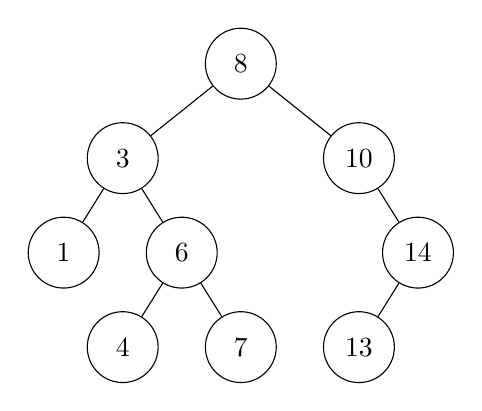
\begin{tikzpicture}[
        every node/.style = {circle, draw, minimum size=0.9cm, font=\normalsize},
        level distance=1.2cm,
        level 1/.style={sibling distance=3cm},
        level 2/.style={sibling distance=1.5cm}
        ]
        \node {8}
            child {node {3}
                child {node {1}}
                child {node {6}
                    child {node {4}}
                    child {node {7}}
                }
            }
            child {node {10}
                child[missing] % No left child for 10, keeps position
                child {node {14}
                    child {node {13}}
                    child[missing] % No right child for 14, keeps position
                }
            };
    \end{tikzpicture}
    \captionof{figure}{Binary search tree}
    \label{fig:binary-tree-example}
\end{figure}

\begin{codeblockmp}[language=C, numbers=none]
struct Node {
    int data;
    struct Node *left;
    struct Node *right;
};
\end{codeblockmp}

\end{minipage}

\vspace{0.5em}

To process all the nodes in a binary tree, \textbf{recursive} traversal is widely used. The main orders are:
\begin{itemize}[noitemsep]
    \item \textbf{Inorder}: Visit the left subtree, then the root, then the right subtree.
    \item \textbf{Preorder}: Visit the root, then the left subtree, then the right subtree.
    \item \textbf{Postorder}: Visit the left subtree, then the right subtree, then the root.
\end{itemize}

\vspace{0.2em}

Below is an example of how to add a new element to a binary search tree:

\vspace{-0.5em}

\begin{codeblock}[language=C]
struct Node* add(struct Node* p, int v) {
    if (p == NULL) { // If the tree is empty, create a new node
        p = (struct Node *) malloc(sizeof *p);
        p->data = v;
        p->left = p->right = NULL;
    }
    // If the value is less than the current node, go left
    else if (v < p->data) {
        p->left = add(p->left, v);
    }
    // If the value is greater than the current node, go right
    else if (v > p->data) {
        p->right = add(p->right, v);
    } else { /* The value is already present, do nothing */ }
    return p;
}
\end{codeblock}

\subsubsection{Advantages and disadvantages}

\textbf{Pros:} Binary search trees (especially if balanced) allow for fast operations: searching, insertion, and deletion are all $O(\log n)$ on average. They also keep data automatically sorted, which makes ordered traversals straightforward.

\textbf{Cons:} If the tree becomes unbalanced (e.g., when many values are inserted in sorted order), performance degrades to $O(n)$. Extra care or specific algorithms are needed to keep it balanced.


\subsection{Hash Tables}

Suppose we have a collection of elements, each associated with a unique key, and we want to efficiently store and retrieve them by key—ideally in constant time. A powerful solution for this is the \textbf{hash table}.

A \textbf{hash table} is a data structure that organizes data based on a computed index, so that insertion, deletion, and lookup operations can be performed very efficiently (typically with average-case $O(1)$ time complexity). Instead of searching through a list, we use a \textit{hash function} to compute an index (or "address") in an array (the "table") where the element should be stored.

The basic idea is as follows:
\begin{itemize}
    \item A \textbf{hash function} transforms a key (which can be a string, number, etc.) into an integer, which is then mapped to one of the available array indices.
    \item Each position in the array is called a \bfit{bucket} or \bfit{slot}.
    \item Ideally, each key maps to a unique index. However, since there are more possible keys than buckets, multiple keys may map to the same index, a situation known as a \textbf{collision}.
    \item To handle collisions, each bucket can store a list (or another structure) of all elements whose keys hash to the same index. This method is known as \textbf{chaining}.
\end{itemize}

\begin{figure}[H]
    \centering
    \includegraphics[width=0.7\textwidth]{assets/hash-table.png}
    \caption{Hash table}
    \label{fig:hash-table}
\end{figure}

\textbf{Pros:} Very fast operations (search, insert, delete) with average $O(1)$ time—performance stays the same even if you have 100 or 10 million elements. The fastest data structure for lookups.

\textbf{Cons:} No ordering: data is scattered pseudo-randomly, so there's no way to print elements in order. Efficiency depends entirely on the quality of the hash function—a poor hash produces lots of collisions and slows everything down.

\newpage

\section{Input and Output}

\subsubsection{Direct Input and Output (I/O) Functions}

In C, not all file operations need to be strictly sequential (from start to end). Sometimes, you need to read or write data at specific positions inside a file—this is known as \bfit{random access} or \textbf{direct I/O}.

Direct I/O functions allow programs to jump to (seek), read from, or write to arbitrary positions in a file. This is especially useful for binary files or large datasets structured in fixed-size records.

Here are the most important functions:

\begin{itemize}
    \item \texttt{fread(void *ptr, size\_t size, size\_t nobj, FILE *stream)}:
    
    Reads up to \plaintt{nobj} objects of size \plaintt{size} from the file referenced by \plaintt{stream} into memory at \plaintt{ptr}. Returns the number of objects actually read (can be less than \plaintt{nobj} at EOF or on error).
    
    \item \texttt{fwrite(const void *ptr, size\_t size, size\_t nobj, FILE *stream)}:
    
    Writes \plaintt{nobj} objects of size \plaintt{size} from memory at \plaintt{ptr} to the file referenced by \plaintt{stream}. Returns the number of objects written.
    
    \item \texttt{fseek(FILE *stream, long offset, int origin)}:
    
    Moves the file position indicator to a given location. \plaintt{origin} can be \plaintt{SEEK\_SET} (beginning), \plaintt{SEEK\_CUR} (current position), or \plaintt{SEEK\_END} (end of file).
    
    \item \texttt{ftell(FILE *stream)}:

    Returns the current position in the file.
    
    \item \texttt{rewind(FILE *stream)}:

    Convenient function to set the file position back to the beginning (same as \plaintt{fseek(stream, 0L, SEEK\_SET)}).
    
    \item \texttt{fgetpos(FILE *stream, fpos\_t *ptr)}, \texttt{fsetpos(FILE *stream, const fpos\_t *ptr)}:

    Save or restore a file position using a special type (\plaintt{fpos\_t}). Useful for marking positions in a file to come back to later.
\end{itemize}

\begin{observationblock}[Sequential vs. Direct Output]
The standard text file operations you may know (\plaintt{fgets}, \plaintt{fprintf}, etc.) always work in order, from start to end. In contrast, direct I/O lets you process files like arrays: you can jump immediately to any position.
\end{observationblock}

\textbf{Example usage:}

\begin{codeblock}[language=C]
/* Write three integers to a binary file */
FILE *fp = fopen("data.bin", "wb");
int arr[3] = {1, 2, 3};
fwrite(arr, sizeof(int), 3, fp);
fclose(fp);

/* Read the second integer only */
fp = fopen("data.bin", "rb");
int x;
fseek(fp, sizeof(int), SEEK_SET); // Skip the first integer
fread(&x, sizeof(int), 1, fp);    // Read the second
printf("%d\n", x);                // Should print 2
fclose(fp);
\end{codeblock}

\textbf{Notes:}
\begin{itemize}
    \item For binary files, direct I/O is safe and efficient.
    \item For text files, random access may not behave as expected due to encoding/newlines—use only when strictly necessary.
    \item Always check the return value of these functions to detect errors or EOF.
\end{itemize}
